\documentclass[12pt]{article}
\usepackage{fullpage}
\usepackage{graphicx, rotating, booktabs} 
\usepackage{times} 
\usepackage{fbb} 
\usepackage{natbib} 
\usepackage{indentfirst} 
\usepackage{setspace}
\usepackage{grffile} 
\usepackage{hyperref}
\usepackage{tikz}
\usepackage[export]{adjustbox}
\usepackage[most]{tcolorbox}
\usepackage{verbatimbox}
\usepackage{lscape}
\usepackage{afterpage}
\usepackage{amsmath}
\usepackage[labelfont={bf},textfont=it,labelsep=period]{caption}
 \usepackage{multirow} 
\setcitestyle{aysep{}}
\usepackage{dcolumn}

\hypersetup{
  colorlinks = true,
  urlcolor = blue,
  linkcolor = black,
  citecolor = black,
  pdfauthor = {Joshua Alley},
  pdfkeywords = {},
  pdftitle = {},
  pdfsubject = {},
  pdfpagemode = UseNone,
%  pdffitwindow = true
%  pdfcenterwindow = true
}



\singlespace
\title{\textbf{Rewarding Commitment: Electoral Cycles in Trade Between Military Allies}}
\author{Joshua Alley \\
Postdoctoral Research Associate \\
University of Virginia\thanks{Thanks to Brian Blankenship, Lauren Peritz, Erik Lin-Greenberg, Zachary Markovitch and participants in the Boston University Political Economy of Security Online Workshop Series for helpful comments.} \\
jkalley@virginia.edu
}

 
\date{\today}

\bibliographystyle{apsr}

\usepackage{sectsty}
\sectionfont{\Large}
\subsectionfont{\noindent\large\textit}
\subsubsectionfont{\normalsize}

\makeatletter
\renewcommand\tiny{\@setfontsize\tiny{9}{10}}
\makeatother


\begin{document}

\maketitle 

\begin{abstract}
How do military alliances impact economic ties?
Protege states have strong incentives to engage in the domestic politics of powerful patrons. 
This paper details how alliance proteges use positive economic statecraft to advance their security by helping committed patron state leaders manipulate the economy during leadership competitions.  
I test these claims with three analyses of trade between the United States and its' allies. 
First, I show that allied states drive electoral cycles in U.S. exports. 
I then show which allies respond more to to elections. 
A subsequent examination of election-year exports from U.S. states shows that increased exports to allies concentrates in swing states, which supports claims that allies tie trade changes to electoral competition.
These results suggest that leaders can employ security commitment for temporary economic and political gains during leadership competitions. 
\end{abstract} 


\newpage 
\doublespace 


\section{Introduction}

%In 2018, a former Obama administration official argued that ``"Trump is trying to conflate his issues over trade and his beef with Europe and the EU with NATO, and he's using our military strength to do that.''\footnote{\url{https://www.usatoday.com/story/news/politics/2018/07/11/donald-trump-complains-trade-europe-nato-summit/774495002/}}
%In 2019, when Donald Trump claimed that ``It's not right to be taken advantage of on NATO and also then to be taken advantage of on trade, and that's what happens,'' he was neither the first nor the last U.S. policymaker to highlight perceived problematic economic concessions to allies.\footnote{\url{https://www.reuters.com/article/us-nato-summit/very-very-nasty-trump-clashes-with-macron-before-nato-summit-idUSKBN1Y7005}}
%Treasury Secretary John Connally claimed in a 1971 speech that the United States ``had the right to expect more equitable trading arrangements'' with its allies (quoted in \citet[pg 175]{Sayle2019}).
%\footnote{See also: \url{https://www.fpri.org/article/2019/04/the-blue-chip-and-the-little-blue-bird-change-and-continuity-in-nato-policy-from-nixon-to-trump/} and \url{https://history.state.gov/historicaldocuments/frus1969-76v03/d155}}
%More recently, Congressional leaders criticized the Biden administration's decision to waive sanctions on the Nord Stream 2 gas pipeline between Russia and Germany.\footnote{\url{https://www.bbc.com/news/world-us-canada-57180674}}


% start with a good story of increased trade near elections 


These examples reflect a general question; can large alliance leaders like the United States translate their preponderant security role into economic influence over junior allies? 
Two schools of thought on economic bargaining in asymmetric alliances give competing answers. 
One argues that alliance patrons have limited economic leverage because they prioritize geopolitical aims \citep{Drezner2013, WolfordKim2017}.
Another perspective claims that alliance leaders have substantial economic influence \citep{Norrlof2010, Brooksetal2013} and threats to reduce security commitment encourage economic concessions \citep[pg. 122]{Oatley2015}. 


I argue that large alliance members' economic leverage depends on leaders' past demonstrations of commitment and prospects for removal.
Leaders who establish a strong alliance commitment reputation are more likely to secure economic concessions during leadership competition, but otherwise have reduced economic leverage.
Small allies will make economic policy changes that help a committed partner retain power without endangering their own tenure in office.  
Thus, leaders who demonstrate alliance commitment are more likely to secure economic concessions during leadership competitions such as elections, but allied policy changes will be temporary and targeted.
When the incumbent leader has shown strong commitment, allies will receive more exports during election years, especially from key electoral constituencies. 
At the same time, prior commitments and elections have no impact of tariffs, as structural concessions endanger allied leaders' domestic political survival. 
Senior allies thus have little economic leverage, unless leadership competition encourages their partners to make economic concessions to bolster their security. 


% Findings
I test three predictions from the argument.
First, I analyze democratic major power trade with junior allied countries. 
I find that when major power leaders signal more support to allied states, trade with allied states increases around elections. 
A subsequent analysis of exports from U.S. states in election years suggests that allies concentrate their imports from the United States in electorally competitive states, which is consistent with strategic economic concessions for leadership competition.
The final analysis shows that unlike trade flows, prior leader commitment and elections have a negligible association with allied tariffs on major power exports. 


% economic and seucrity ties 
The argument and findings address three salient issues in international relations theory and practice. 
First, they speak to debates about how economic and security ties interact \citep{Mastanduno2009, Poast2019}. 
Scholars dispute whether economic linkages drive security ties \citep{BiglaiserDeRouen2007, Fordham2010, Kimball2010}, security concerns encourage economic linkages \citep{Gowa1995, Li2003, LongLeeds2006, GowaMansfield2004}, or both \citep{BiglaiserDeRouen2009, KinneBunte2018}. 
My findings suggest that in some alliances, this relationship changes with leaders' commitment and competition.


% economic cycles
Expanded exports from alliance leaders to junior partners in election years also bolster political business cycles where elites manipulate economic policy to win reelection. 
Elected leaders often use fiscal \citep{Rogoff1987} and monetary policy \citep{ClarkHallerberg2000} to generate economic growth around elections. 
There is also evidence that leaders use non-budget instruments like social policy \citep{Philips2020}, labor agreements \citep{Ahlquist2010}, trade disputes \citep{Conconietal2017} and defense contracts \citep{DerouenHeo2000} to win elections. 
In addition to these domestic mechanisms, other countries can facilitate political budget cycles. 


% coercion
Finally, this paper provides new insight into coercive demands by bridging economic and security bargaining.
When and why coercion succeeds is a salient question (e.g \citep{Sechser2010, Sechser2018, Cebuletal2021}).  
Most studies of coercion examine either security threats (e.g. \citep{HorowitzReiter2001, Sechser2011}) or economic sanctions (e.g. \citep{Marinov2005, Allen2008, Escriba-FolchWright2010}).
This study explores whether security ties provide economic leverage. 
In particular, it assesses issue linkage in alliance management, building on previous work that considers alliance formation \citep{Poast2012} and credibility \citep{Davis2008, Poast2013}. 


% policy 
Whether trade concessions are the price of security alliances also has important implications for how policymakers bargain with allies. 
If threats to reduce security commitments do not lead to economic gains, then they create negative security consequences without economic benefits. 
My findings suggest that alliance skeptics have the least economic leverage, because allies have no incentives to risk domestic disapproval of economic policy changes.
But a cooperative equilibrium where leaders signal support and allies help patron leaders remain in power is possible. 


% need an outline 
The paper proceeds as follows. 
To start, I outline an argument explaining when and why alliance leaders might demand economic concessions from their partners, and when allies might offer economic assistance. 
I then test three predictions from the argument. 
First, I show that U.S. trade balances with allies increase in election years as prior leader signals of support increase. 
I then show that election year exports from the United States to its allies concentrate in swing states. 
Finally, I examine tariff levels and show that allies are unlikely to make structural trade policy changes, even as commitment signals increase. 
The last section discusses the results and offers some concluding thoughts.


\section{Argument}


% basic asymm alliance framework
In asymmetric alliances between large and small states, the large state protects its junior partner in exchange for foreign policy concessions \citep{Morrow1991}.
A credible promise of military support increases the large state's foreign policy influence. 
Small alliance members garner protection from external threats and sacrifice some foreign policy autonomy. 


Military alliances and economic cooperation are inseparable.
Many alliances also include explicit or implicit promises of economic cooperation \citep{GowaMansfield2004, LongLeeds2006, Davis2008, Poast2012}.\footnote{Conflict and economic integration are linked in general (see for example, \citep{GartzkeLi2003, Chen2021}).}
A cooperative bargain of security and economic ties results. 
Although many asymmetric alliance formalize hierarchical relationships, security and economic hierarchy are distinct \citep{Lake2009}, so security preponderance need not secure untrammeled economic influence. 


There are two competing perspectives on the balance of security and economic relations in asymmetric alliances.
One view argues that to prioritize international influence and geopolitical concerns, large state leaders tolerate economic protectionism \citep{Drezner2013, WolfordKim2017}. 
In this perspective, large state leaders prioritize security over economic influence, leaving little economic leverage. 
Another argument holds that large alliance leaders have substantial economic influence \citep{Norrlof2010, Brooksetal2013} and threats to reduce commitment can coerce economic concessions from junior alliance partners \citep{Oatley2015}.  


% overview
I argue that large alliance members usually lack economic leverage, especially when they invest in credible alliance commitments, but allies will make economic changes when a committed patron leader might be replaced. 
This process emphasizes how leaders affect intra-alliance bargaining. 
The way alliances affect economic bargaining depends on leader investment in alliance commitment and leadership competition in the large alliance partner.  
Only leaders with an established reputation for alliance cooperation can leverage security commitments for economic concessions, and only when they or their coalition face competition. 
To uphold alliance security, allies will make temporary economic changes so they support a friendly leader without endangering their own security in office. 


% actors 
There are four key actors in this argument. 
First, the large alliance member leader seeks geopolitical influence and a favorable balance of economic relations. 
Second, a leader in the small alliance member desires security from external threat and a favorable economic balance.
Both leaders are office-seeking and depend on domestic supporters to stay in power.
The third and fourth actors are the domestic actors in both states, who gain or lose from changes in economic ties. 


% economic incentives to retain power
Leaders require domestic support to hold office, and can win support through the distributional consequences of international economic ties. 
Leadership competition through an election or some other leadership challenge increases the pressure on leaders to solidify their coalition or find new supporters. 
Even if a leaders faces term limits, they will often attempt to ensure that their coalition remains in power.  


% goose the economy
Boosting economic prosperity helps leaders increase their odds of retaining office. 
These incentives lead to political business cycles, where leaders manipulate economic policy to increase economic growth and bolster their electoral prospects \citep{Rogoff1987, ClarkHallerberg2000}.
Leaders also use social policy changes to bolster their electoral prospects \citep{Ahlquist2010, Philips2020}. 


% allies can help
Because alliances often support economic ties, allied economic policy can help patron state leaders generate political business cycles. 
Trade, investment and financial ties shape the prosperity of domestic interests.
If large state leaders change the economic bargain in an alliance to the benefit of domestic interests, they increase their odds of retaining power. 


% consider how it works on trad
As an illustration of the domestic political rewards of changing economic relations in an alliance, consider trade politics.
International trade shapes domestic policies, as trade has distributional consequences for domestic interests in large and small alliance members.
Under incomplete trade openness, some domestic sectors in both states are protected from foreign trade competition by tariff or non-tariff barriers. 
Protected sectors have higher incomes than they would under free trade, while sectors with a comparative advantage in the other state lose out on trade income. 


% response: lean on allies for concessions, especially when there's a risk of losing office
There are two domestic political motives for large state leaders to renegotiate the balance of trade and security relations in an alliance. 
First, leaders can increase the income of some domestic sectors.
Increased exports to junior members could benefit domestic interests, who would then back the incumbent. 
Trade expansion also increases domestic consumption and sometimes facilitates intra-industry trade.
Domestic sectors who benefit from increased trade would then be more likely to support the incumbent leader, as trade cleavages shape domestic political coalitions \citep{Rogowski1987, Hiscox2001}. 
 

% BoP 
Trade balances impact the balance of payments between countries.
A negative trade balance creates a current account deficit, which is usually financed with international capital inflows, which further strengthens the currency. 
Increased currency values then make domestic manufacturing and exports less competitive. 
This increases domestic interests' concerns over trade with allies. 


When leaders wish to change economic relations with allies to benefit domestic interests, alliance security guarantees might provide leverage. 
Leaders can renegotiate initial economic arrangements during alliance maintenance. 
Threatening to reconsider their security commitments to smaller partners might increase large state leaders' economic influence. 


% making the threat credible
Credible threats to reduce security commitments in exchange for economic concessions depend on prior alliance investment, however. 
If a leader has not invested in the alliance, their allies have preserve less security by helping them remain in office. 
And if there is no risk of leader turnover, allies have no concern that changes in the ruling coalition will reduce their security. 
Given leadership competition, economic demands contain an implicit threat that rigid economic bargaining might endanger security cooperation by empowering a less committed leader.


% allied incentives to concede- want to keep security, must keep their interests happy too
% new leader might be similar, but less certainty. 
Security threats in economic bargaining create a dilemma for small alliance members. 
Reduced alliance commitments endanger their security, but economic concessions could threaten a leader's hold on office by harming domestic interests. 
Small state leaders thus weigh security benefits of economic policy changes against domestic political consequences.


% security benefits- leader coop
The security benefits of conceding to a patron state leader's economic demands depend on that leader's prior commitment to the alliance. 
In bargaining between allies, reputations for commitment adhere to leaders, who have substantial influence on foreign and economic policy \citep{Renshonetal2018}.
Executive leaders have a pivotal role in decisions to use force (e.g \citep{Colgan2013, ColganWeeks2015}), which are at the heart of alliance politics.
A leader's reputation for alliance cooperation and commitment therefore shapes how allies respond to their economic demands. 
Leaders with a strong commitment reputation extend more security benefits to their allies. 


% need to establish commitment early
When a leader first takes office, only they are fully aware of their commitment to an alliance, so establishing credibility is crucial. 
New leaders' alliance commitment is private information to allies and adversaries. 
Taking costly actions shows whether a leader is committed to the alliance in the same way that new leaders establish a reputation for resolve in crisis bargaining \citep{Wolford2007}. 


Leaders establish alliance commitment by costly signaling \citep{Fearon1997}. 
Hands tying signals through statements of reassurance and commitment to an alliance are one salient way for leaders to establish a cooperative reputation \citep{Blankenship2020}.
Leaders can also sink costs by deploying troops, visiting allied states, offering aid, or undertaking other costly cooperation \citep{McManusNieman2019}.
Both these efforts indicate that a leader is willing to honor alliance promises, as less committed leaders would not make these signals.


% only concede if enough prior res: cooperative reputation
Small alliance member leaders will only make economic concessions if supporting the patron state leader in office offers sufficient security benefits. 
Economic concessions thus depend on the large state leader's cooperative reputation. 
If the large state leader has demonstrated strong commitment to the alliance before making economic demands, then adjusting economic relations to help them retain power is worthwhile.
Small state leaders prefer a cooperative partner to an uncertain leadership or coalition change, given the high stakes of alliance commitments.
If a leader has not tied hands or sunk costs, then allies may be willing to bet on a more invested successor. 
At a minimum, allied states have few incentives to aid a leader who has not invested in their security. 


% prior res establishes rep for restraint too: cebul et al
In addition to establishing that concessions will bolster protege security by helping a friendly leader remain in office, prior cooperation generates a necessary reputation for restraint. 
Committing to not renege and follow through on a threat regardless of cooperation is essential in coercive bargaining \citep{Cebuletal2021}. 
If a leader previously demonstrated commitment to the alliance, it reduces the perceived risk that they will demand further concessions, or reduce security commitment regardless.
This decreases the likelihood of proteges rejecting economic demands to establish a reputation for resolve and ward off future challenges \citep{Sechser2010, Sechser2018}. 


% don't concede too much, however
In addition to commitment reputation, protege leaders face their own domestic political constraints. 
Even when a leader creates a cooperative reputation and faces replacement, domestic concerns constrain allied economic concessions \citep{Davis2008}. 
Trade politics again provides a useful illustration.
Reducing protection for domestic industries or tolerating patron protectionism exposes a leader to domestic political pressure as their industries lose trade income.
Taking down trade barriers is also hard to reverse, especially when states are part of international organizations.
Structural changes increase the risk of a small state leader losing office, so small states will prefer temporary concessions to help cooperative leaders remain in office.
Temporary and targeted measures can help a large state incumbent without antagonizing domestic interests. 
Large states can therefore only leverage security preponderance security role at specific times and in limited ways.


% prior commitment helps in three ways
In trade and other economic areas, I expect that prior commitment provides conditional and limited economic leverage. 
Some concern with leadership change is necessary for commitment to increase patron influence. 
Allies will also make temporary changes instead of adjusting structural policies such as tariffs. 


% early comm, reduced leverage
Commitment signals increase leaders' economic influence when they might be replaced, but reduce it otherwise. 
Investing in security for junior allies makes threats to renegotiate the balance of security and economic relations less credible. 
This mirrors the negative impact of costly peacetime cooperation on junior alliance member military spending \citep{Alley2021isq}.
Moreover, leaders can provide another commitment signal by signaling support and then tolerate the resulting economic protectionism by allies. 
Bearing the costs of allied economic actions is a costly signal of commitment to an alliance because it generates economic inefficiencies. 
It also changes the domestic politics of the protege to support an ongoing alliance \citep{Lake2013}. 


% explains a couple recent things- illustrative
% why'd Biden concede on Nord stream 2? 
Several recent interactions between the United States and its allies help illustrate my claims about economic bargaining in asymmetric alliances. 
First, the Biden administration's controversial decision to waive sanctions and allow completion of the Nord Stream 2 gas pipeline between Germany and Russia support efforts to reassure European allies. 
In addition to allowing this concession to German economic concerns, Biden sought to wind down many of Trump's European trade disputes while talking up the U.S. commitment to NATO and the EU.\footnote{\url{https://www.aljazeera.com/economy/2021/6/15/eu-and-us-call-truce-in-trump-era-trade-war}}


% why did Trump fail to get substantial economic concessions from allies? 
The argument also explains why U.S. allies rarely conceded Donald Trump's trade demands. 
Trump's prior rhetorical attacks on NATO and other U.S. alliances gave allies few incentives help him win re-election. 
Economic concessions might have aided Trump's re-election campaign, in a mirror image of how Chinese soy tariffs reduced Republican vote share in the 2018 midterm election \citep{ChyzhUrbatsch2021}. 
Moreover, Trump sought fundamental trade policy alterations such as reduced barriers to U.S. agricultural products that might have endangered allied leaders' political survival \citep{HeeParkJensen2007}.


% Geographically targeted
In addition to concessions around elections and limited structural change, a third implication of the leadership competition argument is that allies will target their concessions for maximum influence on leadership competition. 
There is ample evidence of such strategic behavior in other domains.
Domestic leaders use targeted trade disputes \citep{Conconietal2017} and defense contracts \citep{DerouenHeo2000} to bolster their electoral prospects in key constituencies.  
Small states have similar incentives to undertake focused economic efforts.
Proteges could target their concessions in crucial electoral districts to bolster a cooperative democratic leader, for instance. 
In autocracies, policy changes could favor members of the leaders' winning coalition, whether by geography or sector.


% allied states
A 2002 trade dispute between the United States and Europe shows that allied states understand how to maximize the electoral implications of their economic policies. 
After George W. Bush imposed tariffs on EU steel to bolster the Republican Party's electoral fortunes in 2002 and 2004, EU retaliatory tariffs hit goods from swing states such as Florida oranges.\footnote{\url{https://www.wsj.com/articles/SB101674938851653120}.}
Faced with lost support in other areas, Bush backed down.\footnote{\url{https://euobserver.com/foreign/13791}}


% the net results 
Large states can therefore only leverage security preponderance for economic influence at specific times and in limited ways.
Protege states will aid political business cycles when a leader has invested in their security. 
Those efforts will not extend to structural concessions that endanger small state domestic interests, however.



\subsection{Implications}



The argument generates several testable implications, especially for democratic alliance leaders.
Elections provide clear markers of leadership competition that allow allies and leaders to their economic bargaining accordingly. 
Open electoral competition also facilitates targeted allied influence on those contests. 


The first hypothesis concerns when and how junior partners make economic concessions. 
Junior partners will adjust trade with allies when the leader facing replacement has demonstrated prior commitment to the alliance. 
Otherwise, junior alliance members may take a chance on elections empowering a more supportive leader. 
Past indicators of commitment include statements of reassurance \citep{Blankenship2020}, aid, troop deployments, defense cooperation \citep{Morrow1994, Alley2021isq} and trade concessions \citep{WolfordKim2017}.


\begin{quote}
\textsc{Economic Change Hypothesis: During election years in a patron state, exports to junior allies will increase as prior commitment signals by the incumbent leader increase.}
\end{quote}



The second hypothesis predicts targeted concessions.
If allies want to support a friendly leader, they may target their economic concessions to crucial regions of electoral contests. 
I test this prediction in the United States, as the Electoral College increases the electoral importance of some states.
Electoral College swing states have a critical role in presidential elections, which encourages U.S. leaders to focus on them in economic policies \citep{KrinerReeves2015, Conconietal2017}.
Therefore, exports from swing states to U.S. allies will increase in the year of elections more than exports from other states.


\begin{quote}
\textsc{Swing States Hypothesis: During presidential election years, exports from states to U.S. allies will increase as electoral competition in that state increases.}
\end{quote}

%
%The third prediction is that economic pressure from larger allies will be more likely when the leader faces replacement through election or some other competition. 
%Given pressure to deliver for domestic interests to remain in office, leaders will be more likely to make economic demands of allies when there is a high chance they will be replaced. 
%These demands are especially likely to cover issues with distributional consequences like trade.
%
%
%\begin{quote}
%\textsc{Economic Demands Hypothesis: As the likelihood of a leadership change increases, leaders of large alliance members will make more economic demands of allies.}
%\end{quote}


The third prediction is that junior allies are unlikely to change their tariff policies. 
Although helping a committed leader remain in office is valuable, the leaders of junior alliance members cannot endanger their own tenure by antagonizing domestic interests.
Therefore, even if a large state leader undertook substantial commitment and faces replacement, their partners will not alter allied tariff schedules. 


\begin{quote}
\textsc{Tariff Hypothesis: During election years in a patron state, tariffs by junior allies will undergo negligible changes, even as prior commitment signals by that leader increase.}
\end{quote}



%\subsection{Objections and Alternative Explanations}
%
%
%% objection- why not dismiss threats/demands by committed leaders as incredible? 
%% stand to benefit from helping them
%Before proceeding examining these hypotheses, I consider two potential objections and alternatives to the argument, including whether committed leaders can make credible economic demands and the role of external threat.
%First, why do junior partners to concede economic demands to committed leaders? 
%While limited concessions are less consequential than tariff changes, they still have costs.
%I expect that the costs of economic concessions support the security benefits of a committed allied leader. 
%Conceding purchases greater security in expectation. 
%
%
%% threat: increases sec demand, but makes it harder to walk away for large partner
%% Cold War should make that fairly clear. 
%Another objection is that increased external threat might make junior alliance partners more receptive to economic demands from their patron.
%Conceding to ensure protection might be worthwhile, in short.
%Though this is plausible, it ignores the incentives of the large partner, who also has more to lose as the threat to junior partners increases. 
%Cold War dynamics illustrate this issue.
%Although the United States initially tolerated and even encouraged European and Japanese protectionism to ensure that allies could rebuild their economies and military capabilities, later efforts to negotiate more favorable trade terms led to substantial resistance from the U.S. security establishment.
%Security leaders feared that U.S. economic nationalism would increase Soviet influence \citep{Mastanduno1998}.
%Threats place pressure on both alliance parties, albeit on different margins.


In the following, I describe how I test each of these hypotheses. 
In the first analysis, I establish that greater commitment by democratic major power leaders increases export to junior allies in election years. 
The second analysis shows that increasing U.S. exports to allied states in election years are concentrated in swing states, which suggests allied concessions concentrate in key electoral constituencies.
Finally, I show that increasing commitment signals do not change protege tariffs on goods from their patron.



\section{Major Power Exports to Allies}

To test the first hypothesis, I analyze democratic major power trade with junior alliance partners. 
I expect that when an election could replace leaders who have signaled greater commitment to their alliance partners, patron state exports to junior partners will increase.
Outside election years, support signals will reduce economic leverage over allies.
This implies a negative constituent term on the leader support variable and a positive interaction between leader signals of support and time to the election.


Following \citet{DigiuseppeShea2021}, I measure leader commitment to each allied state using the latent commitment measure of \citet{McManusNieman2019}, refit to a sample of allied states without the alliance variable. 
Using this measure means that I employ a dyadic dataset of trade relations between the United States, France and United Kingdom and their non-major power allies from 1950 to 2012.\footnote{The analysis stops in 2012 due to limits on the major power support measure.}
Because reputations adhere to leaders, I measure commitment as the moving average of support across each leader's tenure. 
Increased support implies that a leader is more supportive and thus more valuable to allies than likely alternatives.
I then employ elections data from the National Elections across Democracy and Autocracy (NELDA) dataset \citep{HydeMarinov2012} to identify election years.
Finally, I interact the moving average of protege support with a dummy indicator of election years.


The outcome of interest is annual changes in the natural log of exports, but I also model total trade, imports, and the trade balance to assess the net impact of export changes.
Estimating models of changes allows me to include dyadic fixed effects.\footnote{Fixed effects in dynamic models often bias estimates \citep{Nickell1981}. Results are robust to dynamic models without fixed effects. See the appendix for details.}
Furthermore, lagged trade flows have unit roots or near unit root coefficients, so models in levels risk spurious inferences.
I draw on exports and imports data from the IMF's direction of trade statistics database.


In addition to the interaction of time to elections and leader support for allies, I include a series of control variables that may be correlated with alliances and trade. 
%The lagged trade balance addresses temporal autocorrelation in trade ties.
I adjust for changes in the GDP of both states \citep{FouquinHugot2016}, democracy \citep{Marquez2016}, the presence of a militarized interstate dispute \citep{Gibleretal2016}, shared IGO membership \citep{Pevehouseetal2020} and whether an incumbent leader is running.\footnote{Some dyadic data from the \textit{peacesciencer} \textsf{R} package \citep{peacesciencer-package}.}
Finally, I include dummy indicators of years before and after elections.
% population-weighted distance, contiguity, common language, former colonial ties, 


Some trade flow changes are unusual. 
This creates heavy-tailed residuals, so I employ a robust regression estimator; M-estimation with Tukey's biweight function \citep{RaineyBaissa2020}.
Robust regression places less weight on unusual observations, making it more efficient than OLS for this particular outcome.


Dyadic data is also clustered, which can generate misleading regression estimates.
I account for this in two ways. 
First, all models I report here include dyadic fixed effects.
As a result, I estimate the association between leader support, elections and trade within patron-protege dyads. 
Fixed effects estimate within-dyad changes in exports as leader signals of support shift.
Second, I adjust the standard errors for dyadic clustering using the sandwich estimator of \citep{Aronowetal2015}.




\subsection{Results}


As prior support signals by a major power leader increase, exports to non-major power allies increase during election years. 
\autoref{fig:mp-model-coefs} presents coefficient estimates from models of changes in exports, imports, total trade and the trade balance. 
As expected, the interaction between mean leader support and the election year dummy is positive, which implies that leaders who have signaled more support to allies export more to that ally in election years. 
Moreover, the mean leader support signals constituent term is negative in all models, but not clearly so. 
The positive election constituent term is harder to interpret, because it reflects the impact of an election when average leader support is zero and the latent support measure never equals zero. 


\begin{figure}
\centering
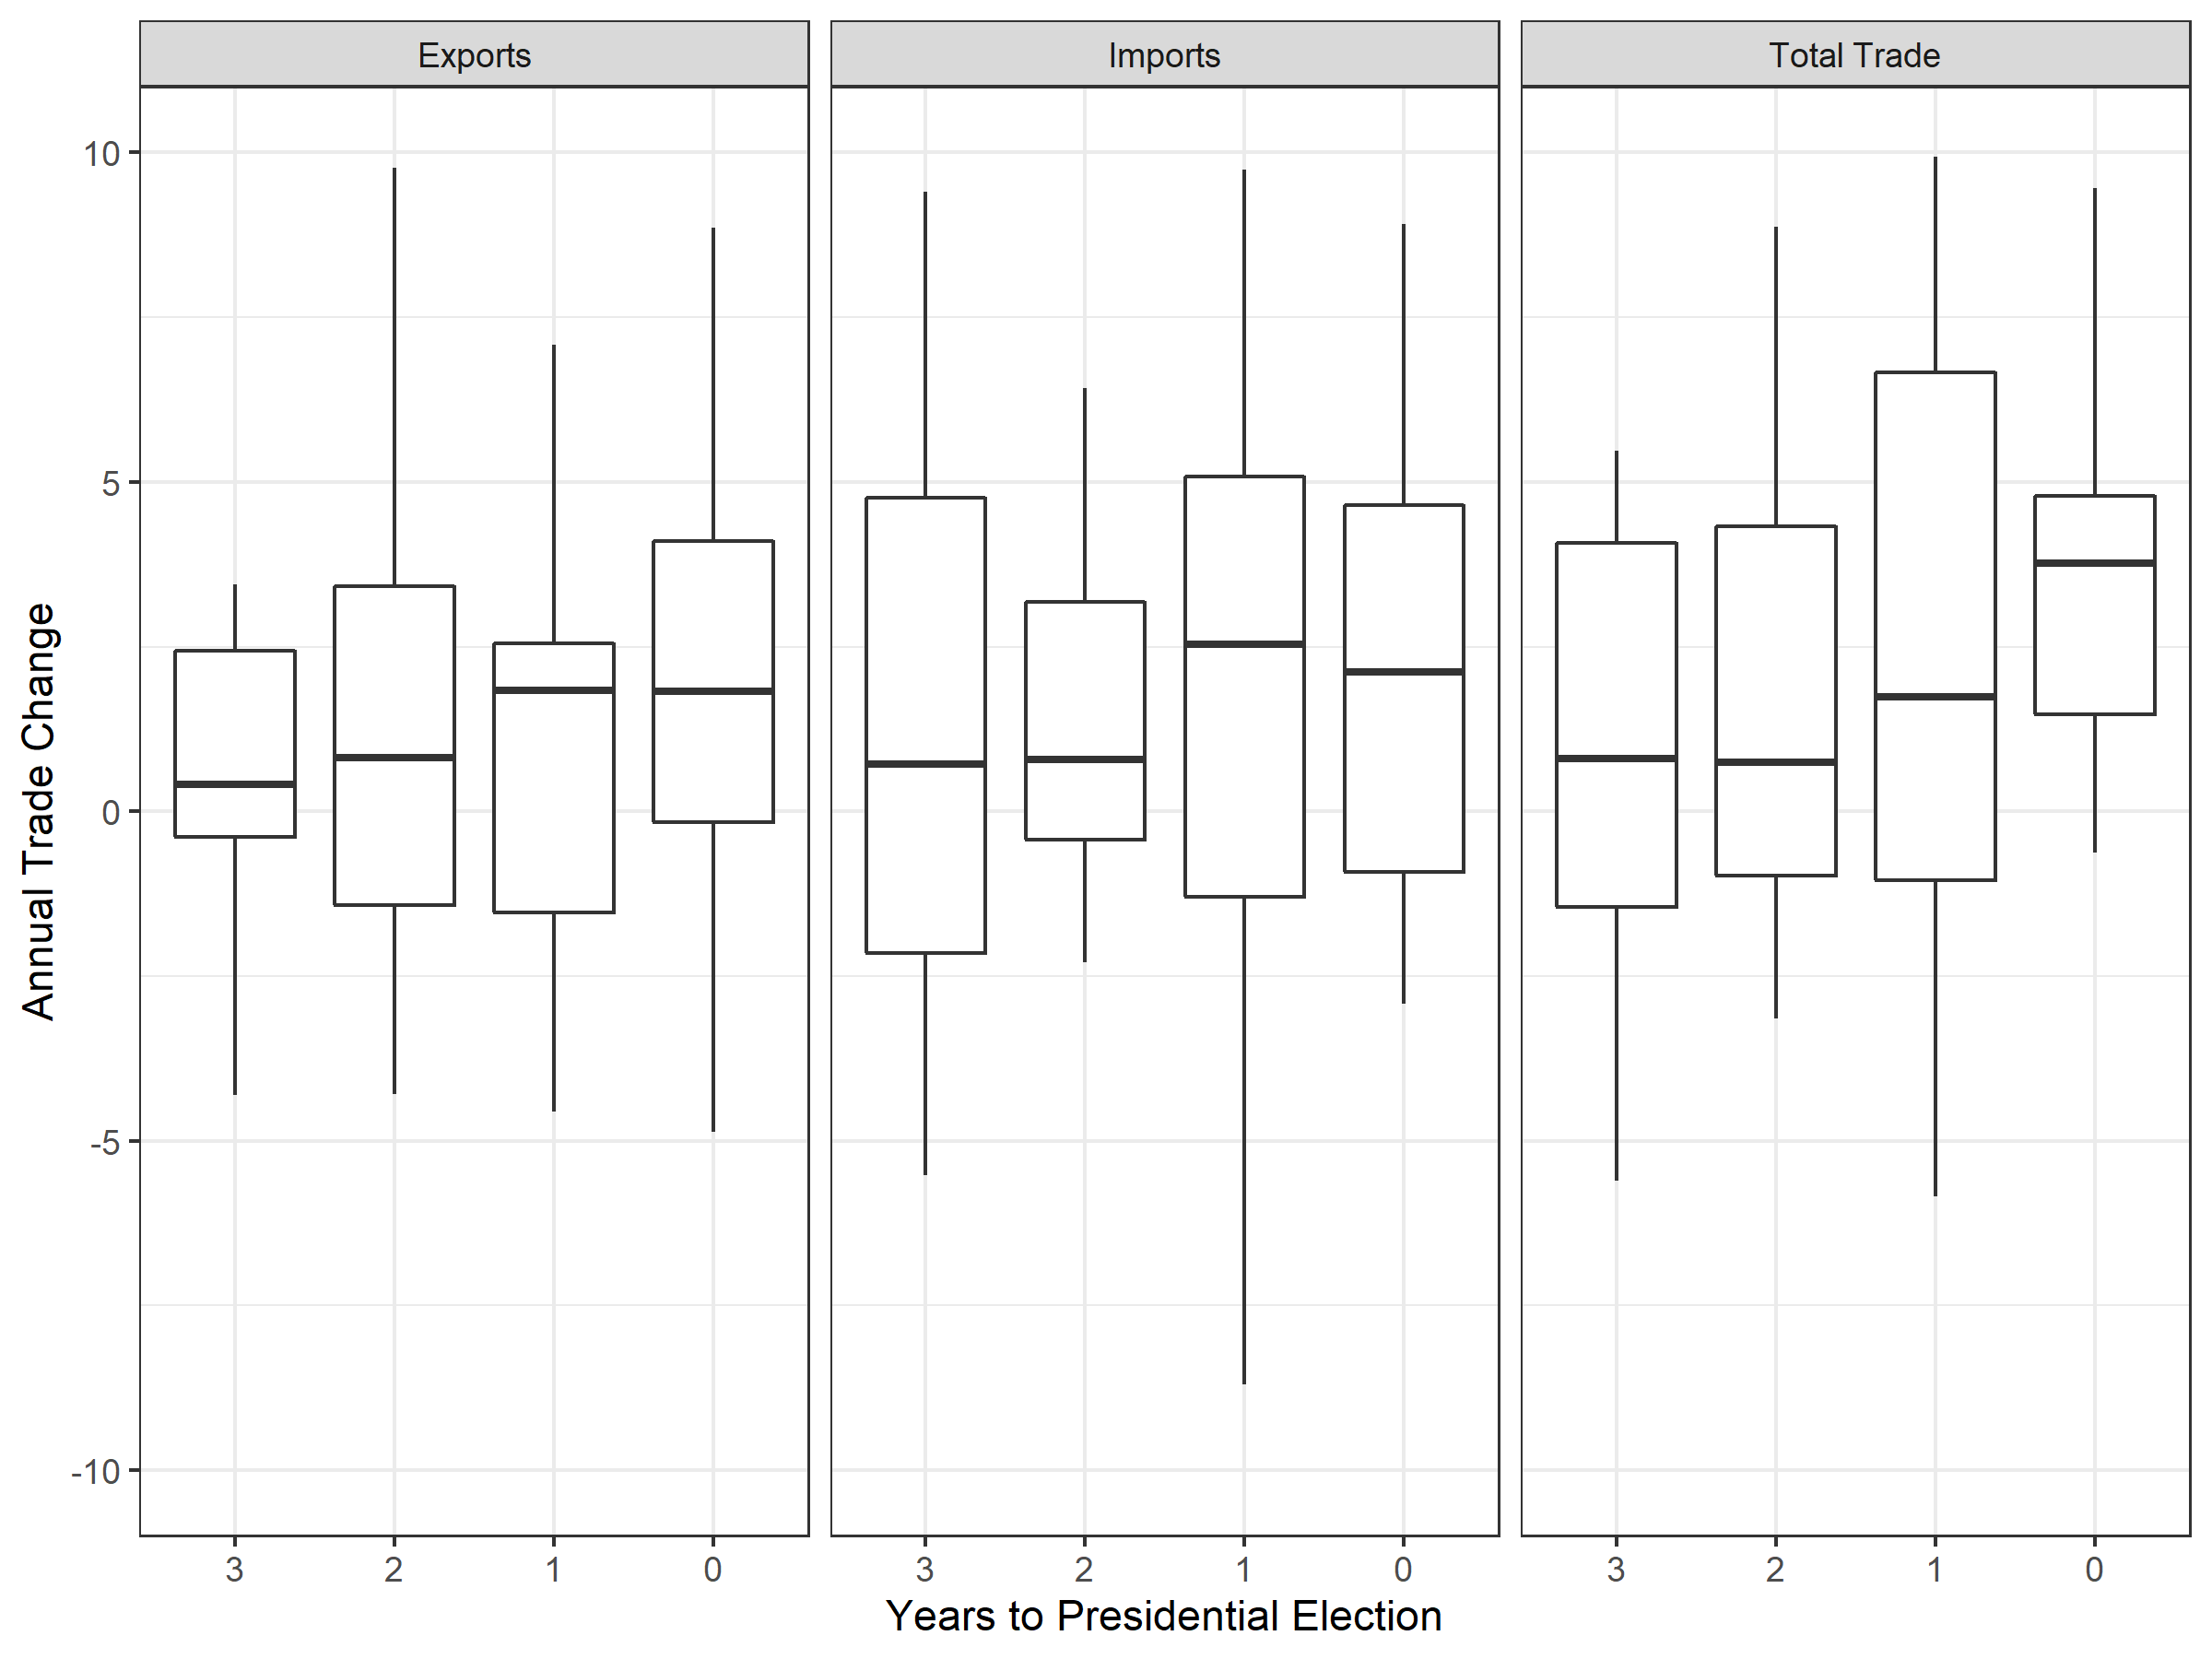
\includegraphics[width=0.95\textwidth]{../figures/us-trade-cycles.png}
\caption{Electoral Cycles in U.S. trade.}
\label{fig:us-trade-cycles}
\end{figure}



% marginal effects
The sign and confidence intervals of the interaction terms are inadequate evidence of a conditional relationship \citep{BramborClarkGolder2006}, so I plot predicted changes in trade flows in \autoref{fig:me-plots-mp}.
This figure presents predicted changes in trade across the range of mean leader support with and without election years. 
Given the non-linear relationships from logged trade flows and a robust estimator, these predictions are more straightforward to interpret than marginal effects.\footnote{I present marginal effects in the appendix.} 


\begin{figure}[htpb]
	\centering
		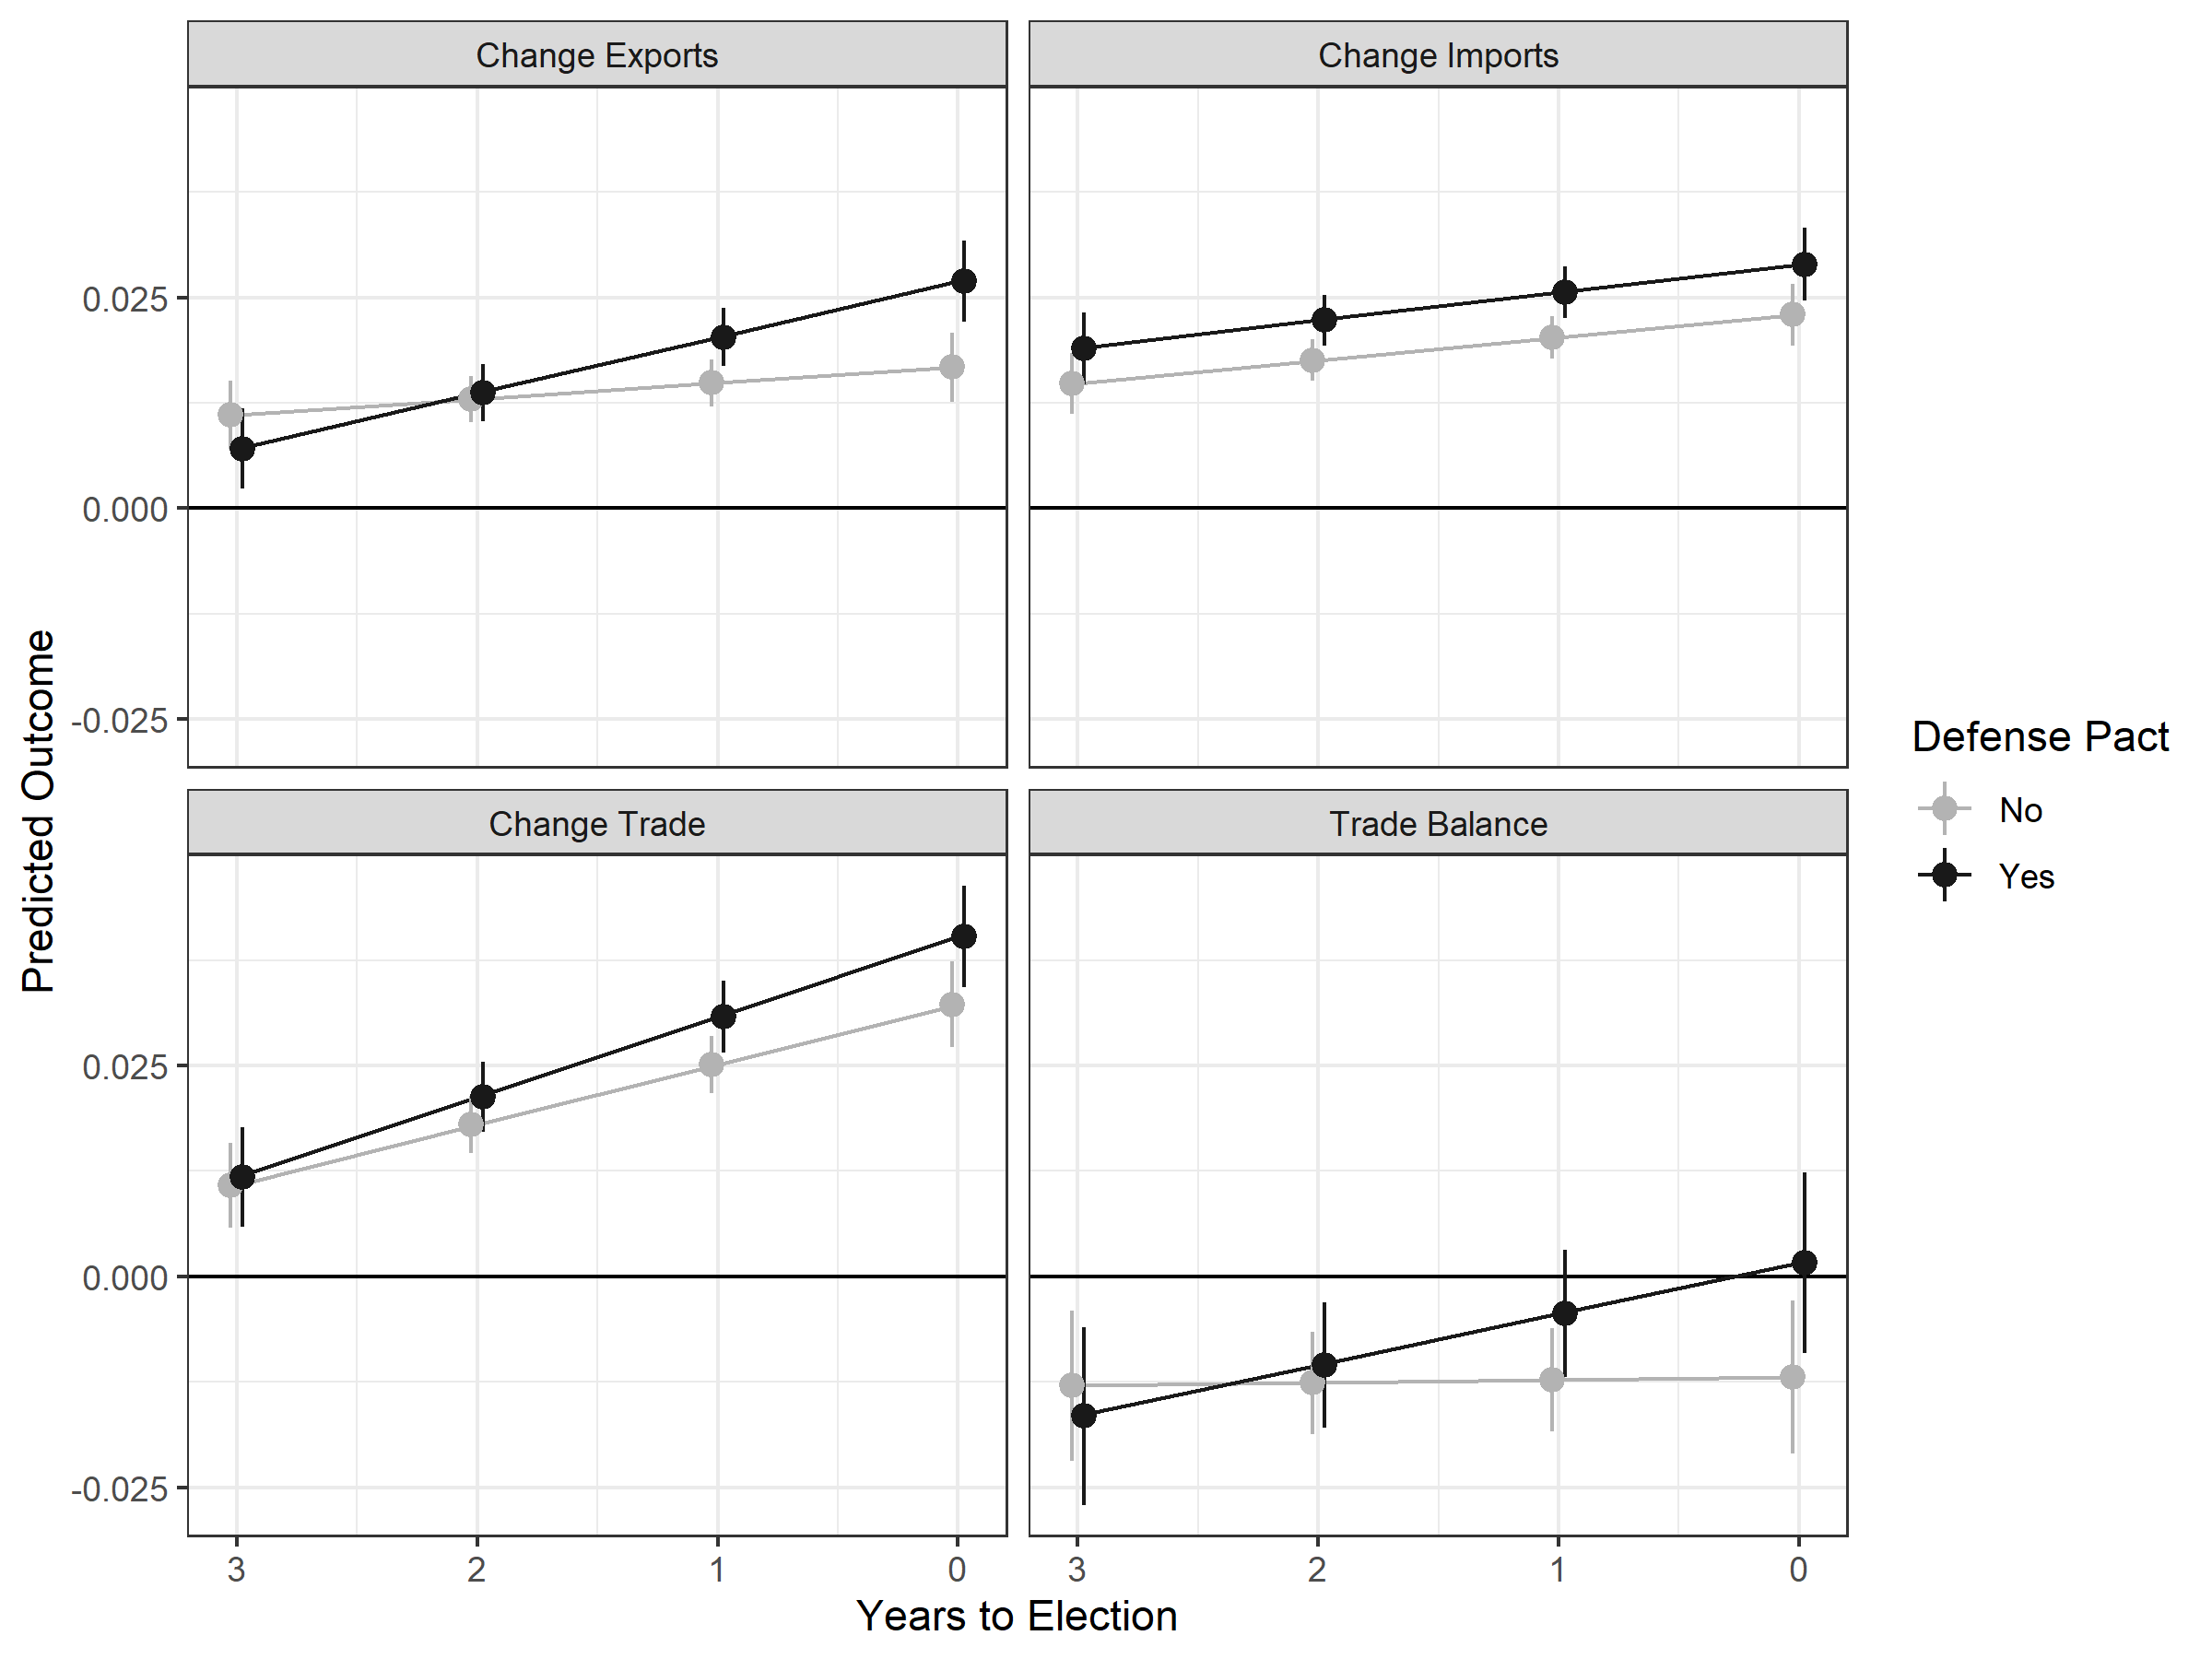
\includegraphics[width=0.95\textwidth]{../figures/us-elec-pred.png}
	\caption{Predicted changes in trade between the the United States and non-major powers. Points lines mark the predictions and error bars summarize the 95\% confidence interval.}
	\label{fig:us-elec-pred}
\end{figure}


The positive interaction between elections and leader support in the model of democratic major power exports reflects a slight increase in exports in election years and falling exports outside of elections. 
In non-election years, greater average support from the incumbent leader reduces major power exports. 
A clear positive difference between election and non-election years at the highest values of mean leader support results. 


% time to election
Imports are less responsive to electoral cycles and leader support. 
A similar pattern might obtain, but predicted imports in election and non-election years at any level of leader support are largely indistinguishable. 
There is a potential difference in total trade, but given limited import fluctuations, this difference is less pronounced than changes in exports. 
Finally, inferences about electoral differences in trade balances across the range of leader support are uncertain.


% control variables show other suggestive evidence of a cycle
Some of the other estimates in \autoref{fig:mp-model-coefs} and \autoref{fig:me-plots-mp} suggest an electoral cycle in democratic major power trade with allies.
Incumbent leaders reduce exports, but democratic major power trade balances with allies also increase before an election.
Furthermore, allied democracy is associated with greater exports from democratic major powers and more positive trade balances.


% improved trade balance
These results are consistent with the economic changes hypothesis. 
When leaders demonstrate alliance commitment, exports to allies are higher in election years than non-election years.
In the next analysis, I show that in the United States, election year exports are concentrated in electorally competitive states.



\section{Swing States and U.S. Exports to Allies in Election Years}


Greater U.S. exports to allied states during election years concentrate in swing states.
In election years, allied states import more goods than other states, especially from important electoral states.
The result holds across two measures of electoral importance--- prior electoral competitiveness and pivot proximity \citep{Wright2009}.


To examine state trade in election years, I fit two gravity models of trade to a dyadic dataset of logged exports from U.S. states to foreign countries during election years.
This analysis employs exports data from the St. Louis Federal Reserve and includes elections from 2002 to 2020.
The key independent variables are a dummy indicator of whether the destination country has a defense pact with the United States and two separate measures of electoral competition. 
Because I expect that allies will be more likely to import from electorally competitive areas to maximize the impact of their economic policy changes, allied imports from swing states should be higher than imports from other states in election years. 
The first electoral competition measure is the difference in the two-party vote share in the last presidential election.
Smaller differences in the vote share imply greater competition.
The second measure captures a state's pivot proximity in the election results. 
The pivot state is the state that, after ranking states by the vote share of the winner, gives the winner 270 electoral votes \citep{Wright2009}.
Keeping the same ranking orders states by distance from the pivot in positive and negative directions--- proximity is the absolute value of this distance. 
Pivot proximity thus encompasses vote share and electoral college considerations. 
A low pivot proximity score implies a state was closer to providing the winning margin and was thus more important, while high proximity distance indicates that a state was unlikely to put the winning candidate over the top.\footnote{To maximize the number of elections in this analysis, I do not examine the conditioning effect of prior leader support, as the latent support measure only runs through 2010.} 


Because smaller pivot proximity and vote differences imply greater competition, I expect that the interaction of U.S. alliance and these variables will be negative, as allied trade with less important states falls off.
The U.S. alliance constituent term should be positive, as alliances support trade most in states with low past vote differences and pivot proximity.
The overall effect of alliances will likely be positive \citep{GowaMansfield2004, Fordham2010}, but it will be strongest in swing states. 
I have no strong expectations about the electoral competition constituent term.


These models adjust for correlates of alliances, electoral competition and trade.
First, standard gravity model controls include the logged population and GDP of each state and corresponding country destination. 
I also adjust for the reelection years of George W. Bush, Barack Obama and Donald Trump with separate dummy indicators, as well as the exchange rate and government spending as a share of GDP in the destination state. 
A lagged dependent variable adjusts for temporal autocorrelation in dyadic exports.
To account for dyadic clustering, especially the diffusion of electoral competition in a state across dyads, I employ a cluster-robust sandwich estimator for the standard errors \citep{Aronowetal2015}.



\subsection{Results}

As expected, allied states import more from U.S. states than other countries during election years. 
U.S. exports to allies also concentrate in electoral college battlegrounds. 
This is consistent with claims that allies make strategic economic concessions. 


\autoref{fig:state-model-coefs} presents the coefficient estimates from the two primary regression models. 
The constituent term for the alliance variable is positive, which indicates that when vote difference is zero, or a state was pivotal in the Electoral College, allied states import more than other states. 
Among non-allied states, electoral salience does not have a clear association with exports. 
The negative interactions between alliances and electoral competition measures indicate that decreasing electoral salience reduces the association between an alliance and exports. 



\begin{figure}[htpb]
	\centering
		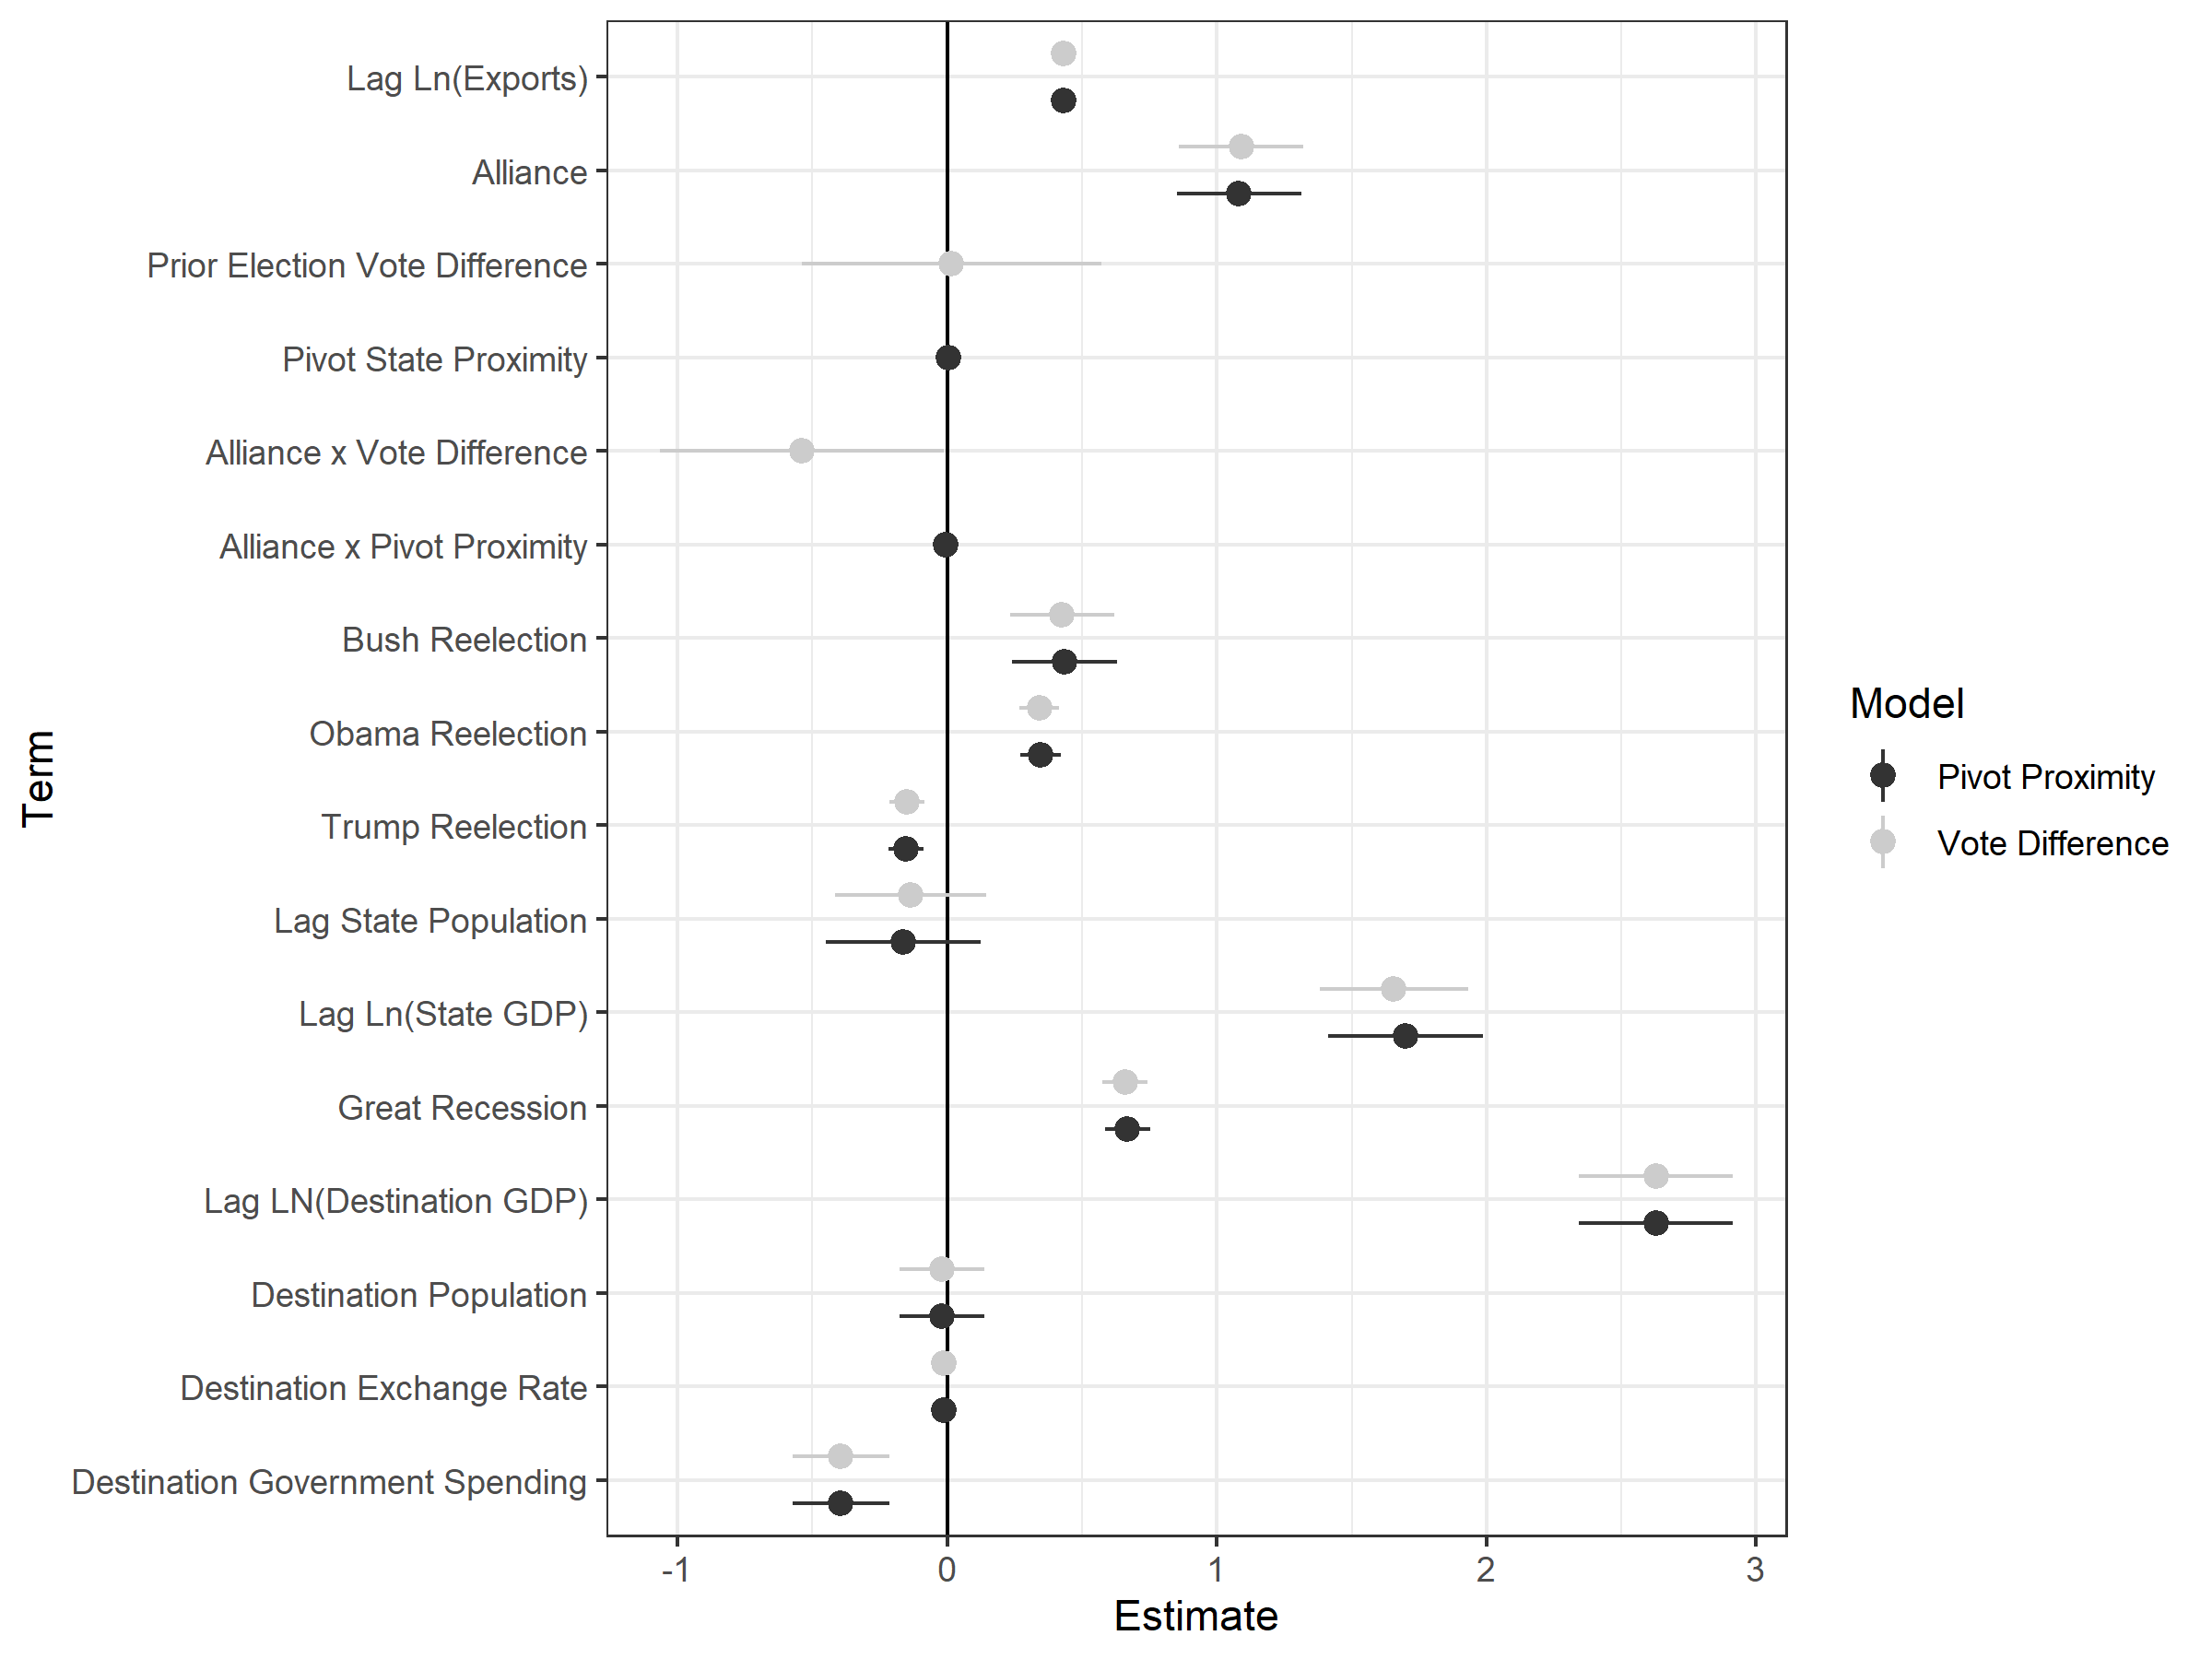
\includegraphics[width=0.95\textwidth]{../figures/state-model-coefs.png}
	\caption{Coefficient estimates from a gravity model of exports from U.S. states to foreign countries, 2002 to 2020. Points mark the coefficient estimates and error bars summarize 95\% confidence intervals.}
	\label{fig:state-model-coefs}
\end{figure}


The control variables in the model are also generally sensible. 
Increasing GDP in the state of origin and international destination both increase exports. 
Trump's 2020 reelection campaign is associated with far lower exports than other elections due to the Covid-19 pandemic. 


To show the interactions, \autoref{fig:me-all-state} presents the estimated marginal effect of an alliance on exports across the range of electoral competition. 
Regardless of prior election vote differences or proximity to the electoral pivot, allies still import more than other states.
The positive association between alliances and trade in election years is stronger in more competitive states, however. 
This implies that allies seek out swing state exports during election years. 


\begin{figure}[htpb]
	\centering
		\includegraphics[width=0.95\textwidth]{../figures/me-all-state.png}
	\caption{Estimated marginal effect of an alliance on exports from U.S. states to foreign countries across two measures of electoral competitiveness, 2002 to 2020. Smaller vote difference or pivot proximity implies greater electoral competition.}
	\label{fig:me-all-state}
\end{figure}


Allies make targeted economic changes in election years. 
U.S. allies concentrate their imports in states that are electorally crucial.
This analysis does not show whether supply or demand drives theses export patterns, however. 
Both paths are plausible. 
Regardless of whether allies seek exports from competitive states, or take on more goods from swing states where politicians want to bolster prosperity to win elections, they faciliate trade flows for electoral advantage. 
%As I show in the appendix, these interactions, as well as the conditional relationship between prior leader support and trade around elections, are robust to alternative interaction specifications and functional forms \citep{Hainmuelleretal2019}.





\section{Discussion and Conclusion}


All three results are consistent with temporary and targeted economic concessions to support committed leaders of large alliance members around elections. 
In the appendix, I check these findings.
First, I check for non-linear relationships and adequate support in the interactions \citep{Hainmuelleretal2019}. 
%I also present inferences from Bayesian models that adjust for dyadic clustering through varying intercepts.
I also present alternative model specifications that find similar conditional relationships.


Demonstrating alliance commitment aids credible security commitments and provides contingent economic leverage. 
Alliance patrons have limited economic leverage, save when allies make temporary economic concessions to help them remain in office. 
Outside of election years, reassuring allies decreases democratic major power exports.
But when leaders offer more support, exports to allies hold up in election years and may concentrate in key constituencies.


Both perspectives on relative economic leverage in asymmetric alliances thus have some validity. 
Demonstrating security commitment often reduces exports and has no impact on allied tariffs. 
At the same time, leaders can leverage security commitments to garner allied support during elections. 


Alliances can therefore help leaders manipulate economic conditions to improve their electoral prospects. 
This finding adds an international mechanism to the political budget cycle literature.
Leaders can use international cooperation in non-economic issues to encourage other states to implement favorable economic policies. 


The argument and results reflect a general phenomenon that is more pronounced in alliances due to close economic and security relations. 
States regularly manipulate international economic ties to bolster or undermine leaders depending on their perceived stance on other issues. 
To give one example, \citet{ChyzhUrbatsch2021} show that Chinese soy tariffs reduced support for Republicans in the 2018 midterm elections. 
Allies have both motive and means to undertake similar actions. 
The security benefits of a cooperative leader motivate economic changes, and allies have many economic ties to leverage when they want to help a friendly leader. 
Future research should examine this phenomenon outside of military alliances.


These results also have implications for democratic alliance credibility and maintenance. 
A stable alliance bargain can develop if leaders anticipate the potential electoral benefits of economic ties with allies.
When leaders expect that demonstrating commitment will have electoral rewards, they will be more likely to invest in alliances. 
This also makes tolerating reduced trade leverage outside of elections worthwhile for patron state leaders.


In addition to assessing how states manipulate economic ties to support friendly leaders, future research could proceed in several directions. 
This paper presents some macro correlations, but could benefit from micro foundations. 
Are individuals more willing to make temporary economic changes that disadvantage domestic firms to support a friendly leader? 
When and how economic ties encourage alliance investments also merits further investigation.
Whether these results generalize to autocratic alliances is another worthwhile inquiry. 


In conclusion, large alliances leaders have limited and conditional economic leverage that depends on political leaders' commitment reputation and leadership competition. 
When a leader makes alliance investments, their exports to allied states increase during election years, and may concentrate in swing states. 
Otherwise, commitment reduces exports, and has no impact on structural policies like tariffs regardless of electoral pressure. 
Security preponderance thus provides less economic leverage than many observers expect, but still grants influence at critical junctures.


\newpage
\singlespace
 
\bibliography{../../MasterBibliography} 


\end{document}